% Copyright 2004 by Till Tantau <tantau@users.sourceforge.net>.
%
% In principle, this file can be redistributed and/or modified under
% the terms of the GNU Public License, version 2.
%
% However, this file is supposed to be a template to be modified
% for your own needs. For this reason, if you use this file as a
% template and not specifically distribute it as part of a another
% package/program, I grant the extra permission to freely copy and
% modify this file as you see fit and even to delete this copyright
% notice. 

\documentclass{beamer}
\usepackage{amsmath}
\usepackage{multirow}
\usepackage{booktabs}

%\newcommand{\tabent}[1]{\makebox[23mm][l]{#1}}
% There are many different themes available for Beamer. A comprehensive
% list with examples is given here:
% http://deic.uab.es/~iblanes/beamer_gallery/index_by_theme.html
% You can uncomment the themes below if you would like to use a different
% one:
%\usetheme{AnnArbor}
%\usetheme{Antibes}
%\usetheme{Bergen}
%\usetheme{Berkeley}
%\usetheme{Berlin}
%\usetheme{Boadilla}
%\usetheme{boxes}
%\usetheme{CambridgeUS}
%\usetheme{Copenhagen}
%\usetheme{Darmstadt}
%\usetheme{default}
%\usetheme{Frankfurt}
%\usetheme{Goettingen}
%\usetheme{Hannover}
%\usetheme{Ilmenau}
%\usetheme{JuanLesPins}
%\usetheme{Luebeck}
\usetheme{Madrid}
%\usetheme{Malmoe}
%\usetheme{Marburg}
%\usetheme{Montpellier}
%\usetheme{PaloAlto}
%\usetheme{Pittsburgh}
%\usetheme{Rochester}
%\usetheme{Singapore}
%\usetheme{Szeged}
%\usetheme{Warsaw}


\makeatother
\setbeamertemplate{footline}
{
  \leavevmode%
  \hbox{%
  \begin{beamercolorbox}[wd=.3\paperwidth,ht=2.25ex,dp=1ex,center]{author in head/foot}%
    \usebeamerfont{author in head/foot}Ziying Yang
  \end{beamercolorbox}%
  \begin{beamercolorbox}[wd=.7\paperwidth,ht=2.25ex,dp=1ex,center]{title in head/foot}%
    \usebeamerfont{title in head/foot}\insertshorttitle\hspace*{3em}
    \insertframenumber{} / \inserttotalframenumber\hspace*{1ex}
  \end{beamercolorbox}}%
  \vskip0pt%
}
\makeatletter
\setbeamertemplate{navigation symbols}{}

\title{How Precise Does Document Scoring Need To Be?}

% A subtitle is optional and this may be deleted
%\subtitle{Optional Subtitle}

\author{\textbf{Ziying Yang}, Alistair Moffat, and Andrew Turpin}
% - Give the names in the same order as the appear in the paper.
% - Use the \inst{?} command only if the authors have different
%   affiliation.

\institute[Universities of Melbourne] % (optional, but mostly needed)
{
  \inst{}%
  University of Melbourne
}
% - Use the \inst command only if there are several affiliations.
% - Keep it simple, no one is interested in your street address.

\date{}
% - Either use conference name or its abbreviation.
% - Not really informative to the audience, more for people (including
%   yourself) who are reading the slides online

\subject{Master Project Presentation}
% This is only inserted into the PDF information catalog. Can be left
% out. 

% If you have a file called "university-logo-filename.xxx", where xxx
% is a graphic format that can be processed by latex or pdflatex,
% resp., then you can add a logo as follows:

% \pgfdeclareimage[height=0.5cm]{university-logo}{university-logo-filename}
% \logo{\pgfuseimage{university-logo}}

% Delete this, if you do not want the table of contents to pop up at
% the beginning of each subsection:

%\AtBeginSubsection[]
%{
%  \begin{frame}<beamer>{Outline}
%    \tableofcontents[currentsection,currentsubsection]
%  \end{frame}
%}

% Let's get started
\begin{document}

\begin{frame}
  \titlepage
\end{frame}

% Section and subsections will appear in the presentation overview
% and table of contents.
\section{Introduction}
\begin{frame}{Background -- Batch Evaluation Technique}
\begin{block}{Question}
\\[0.3em]
\textit{Is IR System A demonstrably better than IR System B?}
\end{block}
\pause
\\[1em]
For each of system A and B\\[0.4em]
\begin{itemize}
  \item For each of a set of topics
  \begin{itemize}
    \item Compute the \alert{similarity score} relative to the topic for each document
    \item Generate a run in decreasing score order
    \item Evaluate the run via relevance judgments and an effectiveness metric
    \item Generate a \alert{run score} for that system and topic
  \end{itemize}
  \pause
  \item Aggregate run scores over the set of topics into a single \alert{system score}\\[1em] 
  %seemed as the overall performance quality of the system
\end{itemize}

We then compare system A and B using their system scores.
\end{frame}

\section{Ties}
\begin{frame}{How to Deal with Tied Similarity Scores?}

Effectiveness metrics use {\color{blue}ranks}, not {\color{blue}similarity scores}.\\[1.5em]

Ties: when more than two items receive the same scores.\\[1.5em]

How should \alert{similarity score ties} be handled?\\[1.5em]
%explain what is ties

{\color{blue}Different orderings} of tied documents may lead to {\color{blue}different system scores}, and might influence the outcome of the experiment.
% \begin{itemize}
%   \item We evaluate TREC-8 runs to determine the impact of tied scores
%   \item Any permutation of tied documents ordering can be presented to the user.
%   %\item Possible treatments: Pick an arbitrary ranking? Order them by document ID?
% \end{itemize}
\end{frame}
\begin{frame}{How to Deal with Tied Similarity Scores?}
\uncover<1->{\begin{block}{Example}
\begin{tabular}{l|@{\hspace{1.5em}} *{7}{l@{\hspace{1.8em}}}}
\tabent{rank, $k$}
  & 1
      & 2
        & 3
        & 4
          & 5
                & 6
            & 7
\\
\hline
\tabent{document, $d_k$}
  & D
      & H
          & A
        & C
            & M
          & S
              & W
\\
\tabent{gain, $r_k$}
  & 0
      & 0
          & 1
        & 1
            & 0
          & 1
              & 1
\\
\tabent{similarity score}
  & 9.8
      & \alert{9.3}
          & \alert{9.3}
        & \alert{9.3}
            & {\color{blue}8.4}
          & {\color{blue}8.4}
              & 8.2
% \\
% \tabent{groups}
%   & \multicolumn{1}{@{}l}{$b_1{=}1$}
%       & \multicolumn{1}{@{}l}{$b_2{=}2$}
%           &
%         &
%             & \multicolumn{1}{@{}l}{$b_3{=}5$}
%           &
%               & \multicolumn{1}{@{}l}{$b_4{=}7$}
\end{tabular}
\end{block}}
\only<1>{
Divide the ranking of a run into \alert{groups} in which the documents have the same similarity score\\[3.2em]
%Denote \alert{$b_g$} as the beginning rank of the \alert{$g$th} group.
}
\uncover<2->{Possible methods for dealing with ties in the run:
\begin{itemize}
\uncover<2->{\item {\color{blue}Run Order}
  \only<2>{: ignore the similarity score, use the presented ordering. (RBP$0.5=0.211$)\\[4.5em]}\only<3->{(RBP$0.5=0.211$)}}
\uncover<3->{\item {\color{blue}External Tie-Break Rule}
  \only<3>{: re-order tied documents in each group using fixed ordering criterion, such as sorting by document ID (\texttt{trec\_eval} program), filename, length and so on. (RBP$0.5=0.227$)\\[3.2em]}\only<4->{(RBP$0.5=0.227$)} }

\uncover<4->{\item {\color{blue}Limits}
  \only<4>{: compute the best and worst run scores that may arise and present a score range instead of a single score value. (RBP$0.5 = [0.211,0.414]$)\\[3.2em]} \only<5->{(RBP$0.5 = [0.211,0.414]$)}}

\uncover<5->{\item {\color{blue}Averaging Across Permutations}
  \only<5>{: compute the average run score across all possible permutations of documents in each group. (RBP$0.5 = 0.323$)\\[3.2em]}}
\end{itemize}}
\end{frame}

\begin{frame}{Ties in TREC Experimentation}
To explore the role of ties in TREC evaluation, we re-sorted the TREC7 submissions, using decreasing {\color{blue}similarity score} as a {\color{blue}primary key}, and increasing {\color{blue}rank} as a {\color{blue}secondary key}.

\begin{table}
\caption{The percentage of \alert{103} systems, \alert{50 $\times$ 103} runs and \alert{4,900,042} documents affected by ties occurring in TREC7 Ad--Hoc runs after score-based re-sorting}
\begin{tabular}{l c ccc}
%\toprule
%  && \multicolumn{3}{c}{Percentage affected}
%\\
%\cmidrule{3-5}
  && systems
    & runs
      & documents
\\
\midrule
Tied similarity scores
  && 95.2\%
    & 91.0\%
      & 14.0\%
\\
Rank/score contradictions
  && \D6.8\%
    & \D4.2\%
      & \D1.4\%
\\
%\bottomrule
\end{tabular}
\end{table}
\end{frame}

\begin{frame}{Ties in TREC Experimentation}
Examine the effect of ties on AP scores for systems
\begin{itemize}
  \item For each system, calculate {\color{blue}mean AP} score over 50 topics using {\color{blue}\texttt{trec\_eval}}.
  \item Select the top 80 systems, as ordered by mean AP score.
  \item For each selected system, compute
  \begin{itemize}
    \item Run Order: {\color{blue}mean} (across topics) of the AP score (by {\color{blue}\texttt{trec\_eval}}).
    \item Limits: {\color{blue}mean} (across topics) of the {\color{blue}best} and {\color{blue}worst} AP score.
    \item Permuations: {\color{blue}mean} (across topics) of the {\color{blue}average} (across permutations of the tied groups in the run) AP score.
    
  \end{itemize}

\end{itemize}
\end{frame}

\begin{frame}{Imprecision in AP Scores Caused by Ties}
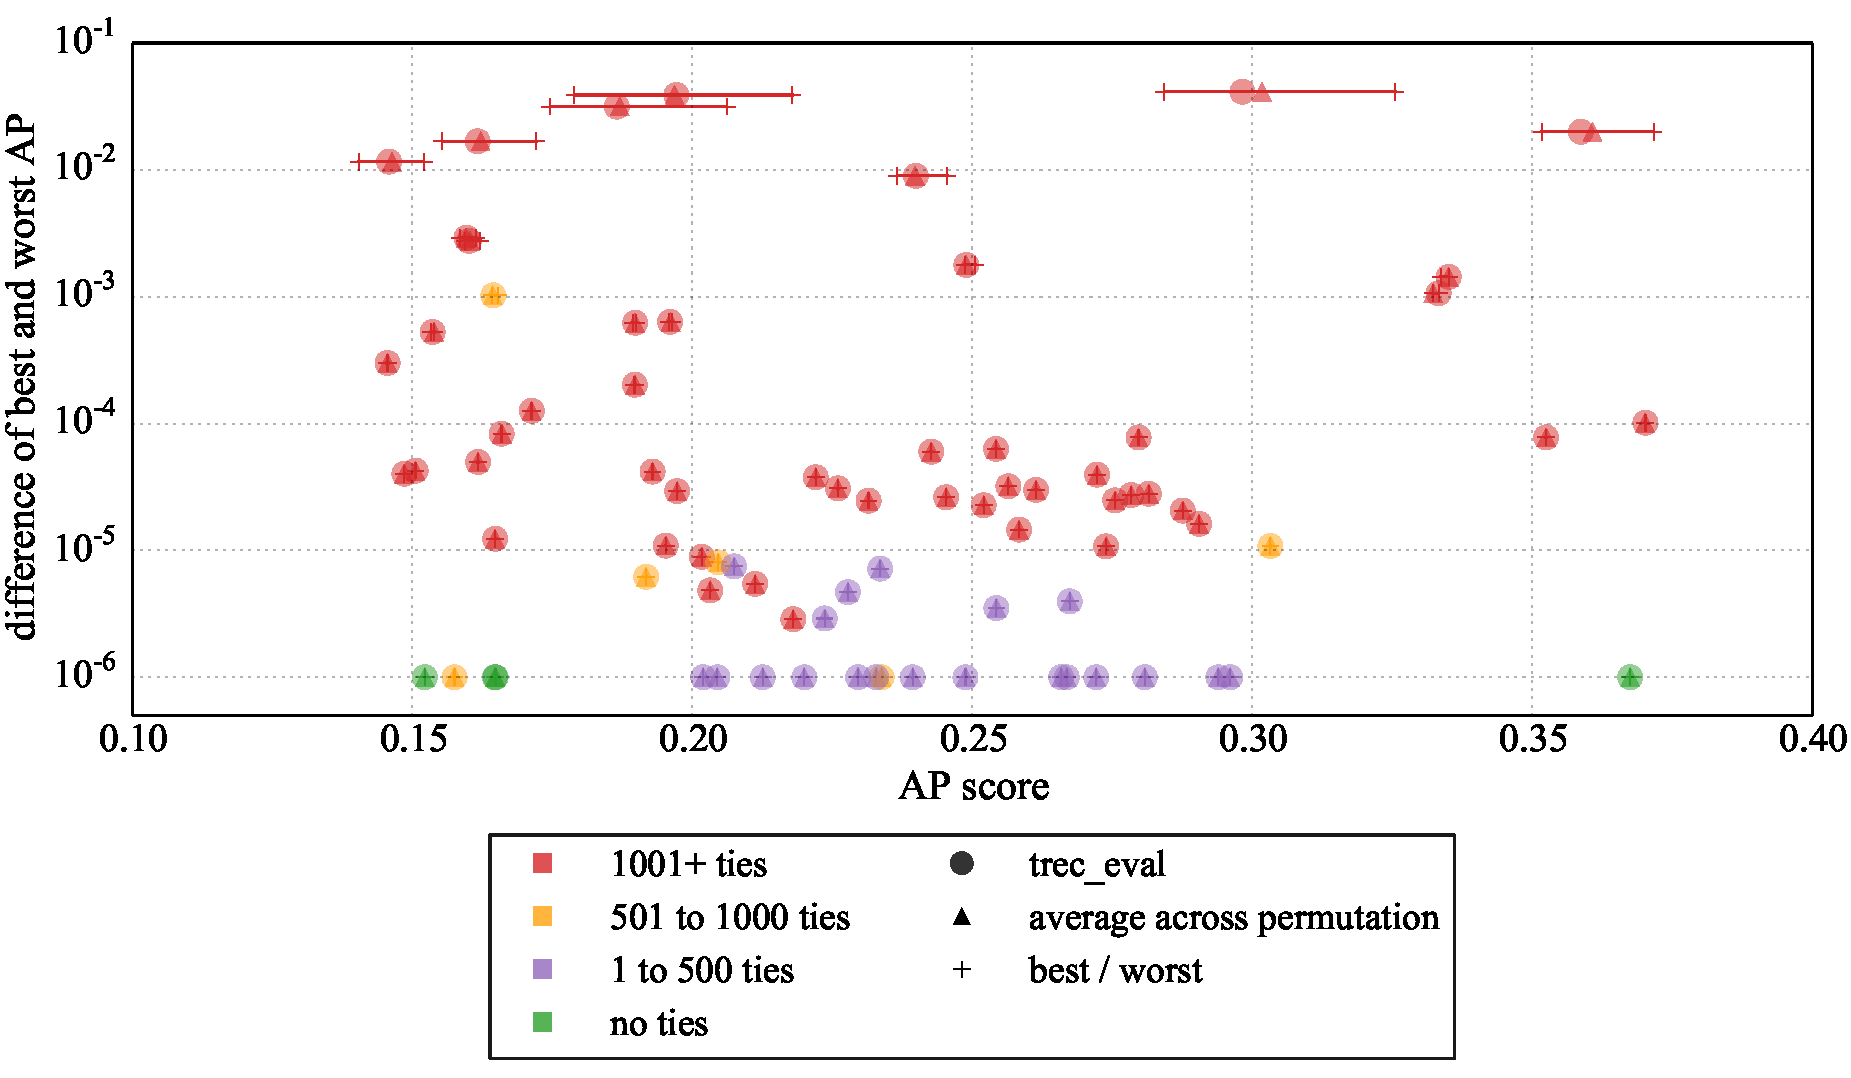
\includegraphics[width=0.98\textwidth]{figs/fig-trec7-ap-scores.pdf}
\end{frame}

\section{Deliberate Score Grouping}
\begin{frame}{Similarity Score Rounding}
%We showed that tied scores had the potential to be disruptive to TREC evaluation, but in practical turns did not. \\[1.5em]

Ties may have been caused by {\color{blue}similarity score rounding}. \\[1em]

\begin{block}{Question}
\textit{Do documents really need to assign similarity scores with high accuracy? How much similarity score rounding can be tolerated without greatly affecting system comparisons?}
\end{block}
\\[1em]
The finding offers the potential for {\color{blue}approximate scoring regimes} that provide {\color{blue}faster search} with little or no loss of effectiveness.

\end{frame}

\begin{frame}{Deliberate Similarity Score Grouping}
Will the deliberate use of ties affect retrieval quality?\\[1em]

Documents are scored and assigned in \alert{bands} of the ranking. Bands are defined geometrically based on a parameter \alert{$\rho$} ($\rho > 1$). More precisely:\\[0.5em]

For the \alert{$g$th} band:
\begin{itemize}
\item the begining rank: $b_g = \lceil{\rho\cdot b_{g-1}}\rceil$, $b_1 = 1$.
\item the ending rank: $e_g = b_{g+1}-1$\\[0.5em]
\end{itemize}
For example:\\
if \alert{$\rho = 2$}\\[0.3em] \text{ } 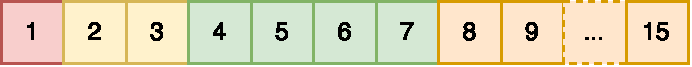
\includegraphics{figs/grouping_exp_rho2.pdf}\\
if \alert{$\rho=1.62$} (the golden ratio)\\[0.3em] \text{ } 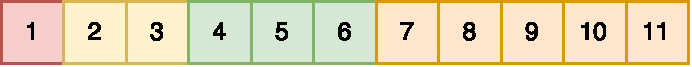
\includegraphics{figs/grouping_exp_rho162.pdf}
\end{frame}

%-----the run concept changed-----

\begin{frame}{Run Score Differences in Practice}
  For each of the $80 \times 50$ system--topic runs 
  \begin{itemize}
  \item compute effectiveness scores of metrics RR, RBP0.5, RBP0.85 and AP using the {\color{blue}original run}
  \item map original run to a banded ranking list using a $\rho$
  \item score the {\color{blue}banded run} using same metrics\\[1em]
  \end{itemize}
  Compute $80 \times 50$ run score differences.
\end{frame}


\begin{frame}{Variation in Run Score of AP}
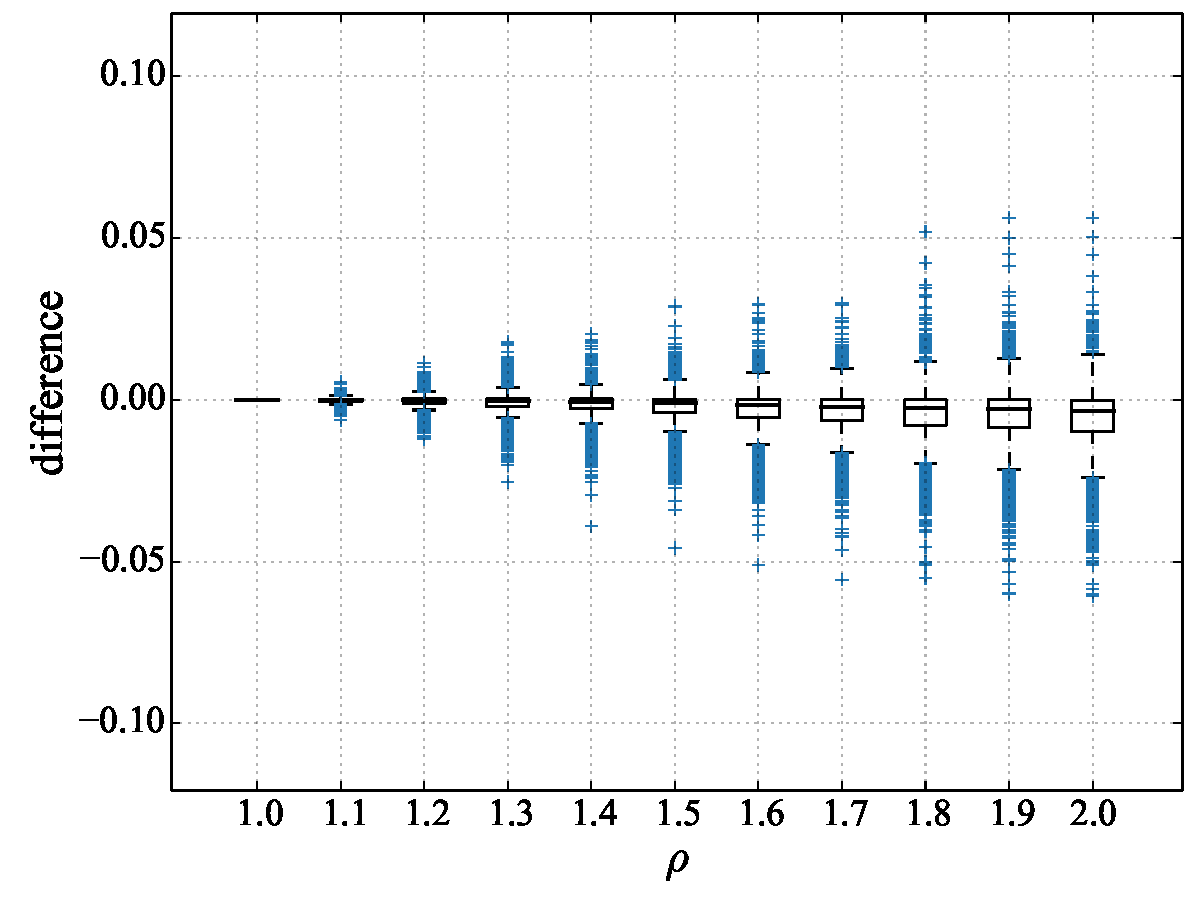
\includegraphics[width=0.9\textwidth]{figs/fig-score-variation-ap.pdf}
\end{frame}

\begin{frame}{Variation in Run Score of RBP ($p = 0.85$)}
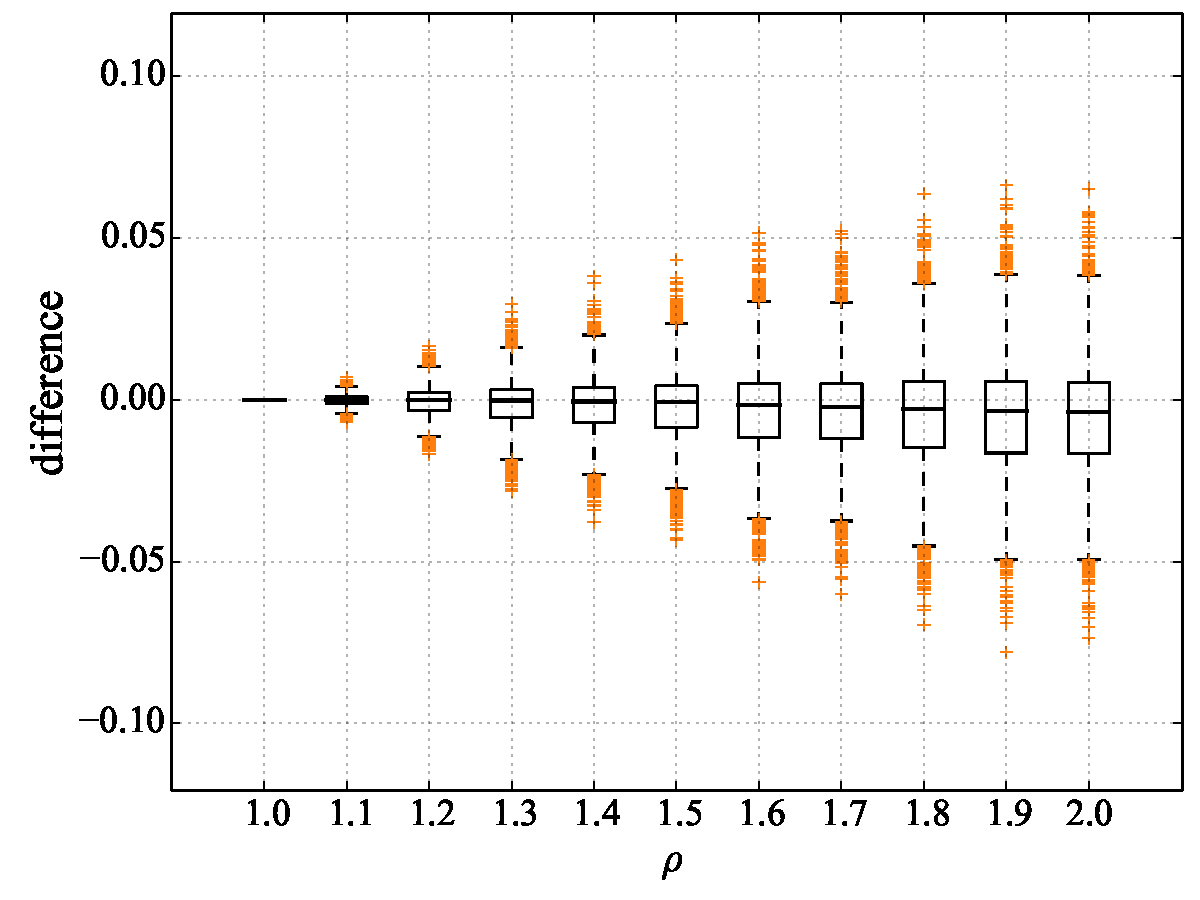
\includegraphics[width=0.9\textwidth]{figs/fig-score-variation-rbp85.pdf}
\end{frame}

\begin{frame}{Variation in Run Score of RBP ($p = 0.5$)}
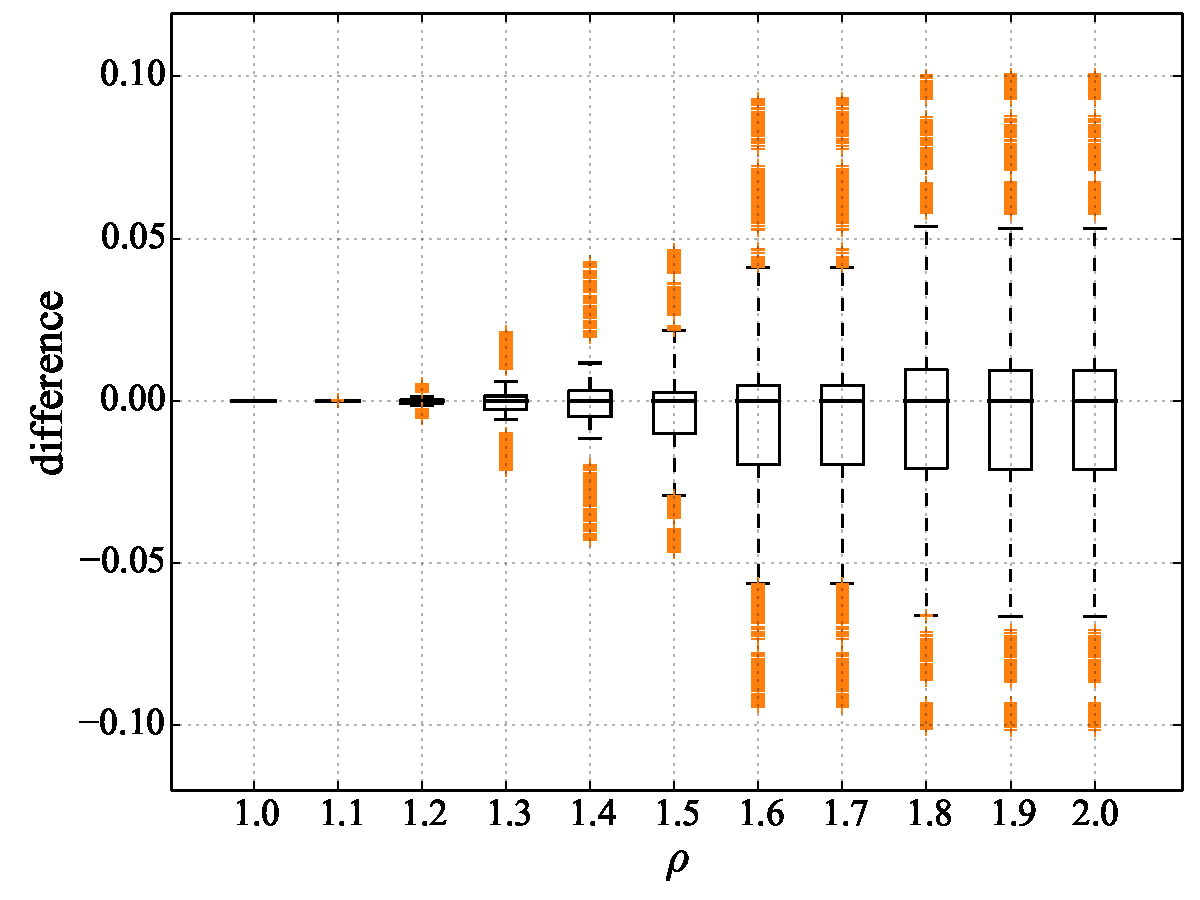
\includegraphics[width=0.9\textwidth]{figs/fig-score-variation-rbp50.pdf}
\end{frame}

\begin{frame}{Are the Differences Significant?}
%The differences of scores seem small, but it can still be significant.

Using the one-tail paired $t$--test, compare the {\color{blue}banded run scores} to the {\color{blue}original run scores $\times$ 97\%}\\[1.5em]

Number of systems (max. 80) for which a $t$--test across 50 topics yields confidence at the $p \leq 0.05$ that the banded run score greater than or equal to 97\% of the original run score.

\begin{table}
\newcommand{\tabent}[1]{\makebox[15mm][c]{#1}}
\begin{tabular}{l c cccc}
\toprule
\multirow{2}{*}{$\rho$}
%  && \multicolumn{4}{c}{Relative to $99$\% of original score}
    && \multicolumn{4}{c}{Relative to $97$\% of original run score}
\\
\cmidrule{3-6}%\cmidrule{8-11}
  % && \tabent{RR}
  %   & \tabent{RBP0.5}
  %     & \tabent{RBP0.85}
  %       & \tabent{AP}
          && \tabent{RR}
            & \tabent{RBP0.5}
              & \tabent{RBP0.85}
                & \tabent{AP}
\\
\midrule
1.1
  % && 80
  %   & 80
  %     & 80
  %       & 80
          && 80
            & 80
              & 80
                & 80
\\
1.2
  % && 80
  %   & 80
  %     & 80
  %       & 80
          && 80
            & 80
              & 80
                & 80
\\
%% 1.3
%%  && 80
%%    & 79
%%      & 76
%%        & 73
%%          && 80
%%            & 80
%%              & 80
%%                & 80
%% \\
1.4
  % && 77
  %   & 44
  %     & 65
  %       & 44
          && 80
            & 80
              & 80
                & 80
\\
%% 1.5
%%  && 73
%%    & 40
%%      & 44
%%        & 7
%%          && 80
%%            & 80
%%              & 80
%%                & 80
%% \\
%% 1.6
%%  && 38
%%    & 11
%%      & 15
%%        & 1
%%          && 80
%%            & 67
%%              & 80
%%                & 80
%% \\
1.7
  % && 37
  %   & 11
  %     & 14
  %       &\D0
          && 80
            & 67
              & 80
                & 77
\\
%% 1.8
%%  && 38
%%    & 10
%%      & 5
%%        & 0
%%          && 80
%%            & 61
%%              & 77
%%                & 60
%% \\
%% 1.9
%%  && 39
%%    & 10
%%      & 3
%%        & 0
%%          && 80
%%            & 61
%%              & 72
%%                & 43
%% \\
2.0
  % && 38
  %   & 10
  %     &\D3
  %       &\D0
          && 80
            & 61
              & 71
                & 20
\\
\bottomrule
\end{tabular}

\end{table}
\end{frame}

\begin{frame}{System Comparison Sensitivity}
Compare systems in pairwise to explore the {\color{blue}implications} that the {\color{blue}similarity score rounding} has on ability the metrics to {\color{blue}differentiate} systems.\\[1.7em]

Perform the paired $t$--test using the {\color{blue}original runs} and {\color{blue}grouped runs} with different value of $\rho$:
\begin{itemize}
\item Generate \alert{$80 \times 79 / 2$ system pairs} 
\item Use their run scores given by metrics
\item Explore the \alert{null hypothesis}: two systems in a pair are same
\item Check if the generated \alert{$p \leq 0.05$}
\end{itemize}
 
\end{frame}

\begin{frame}{Correlation of $p$ Values for All System Pairs}
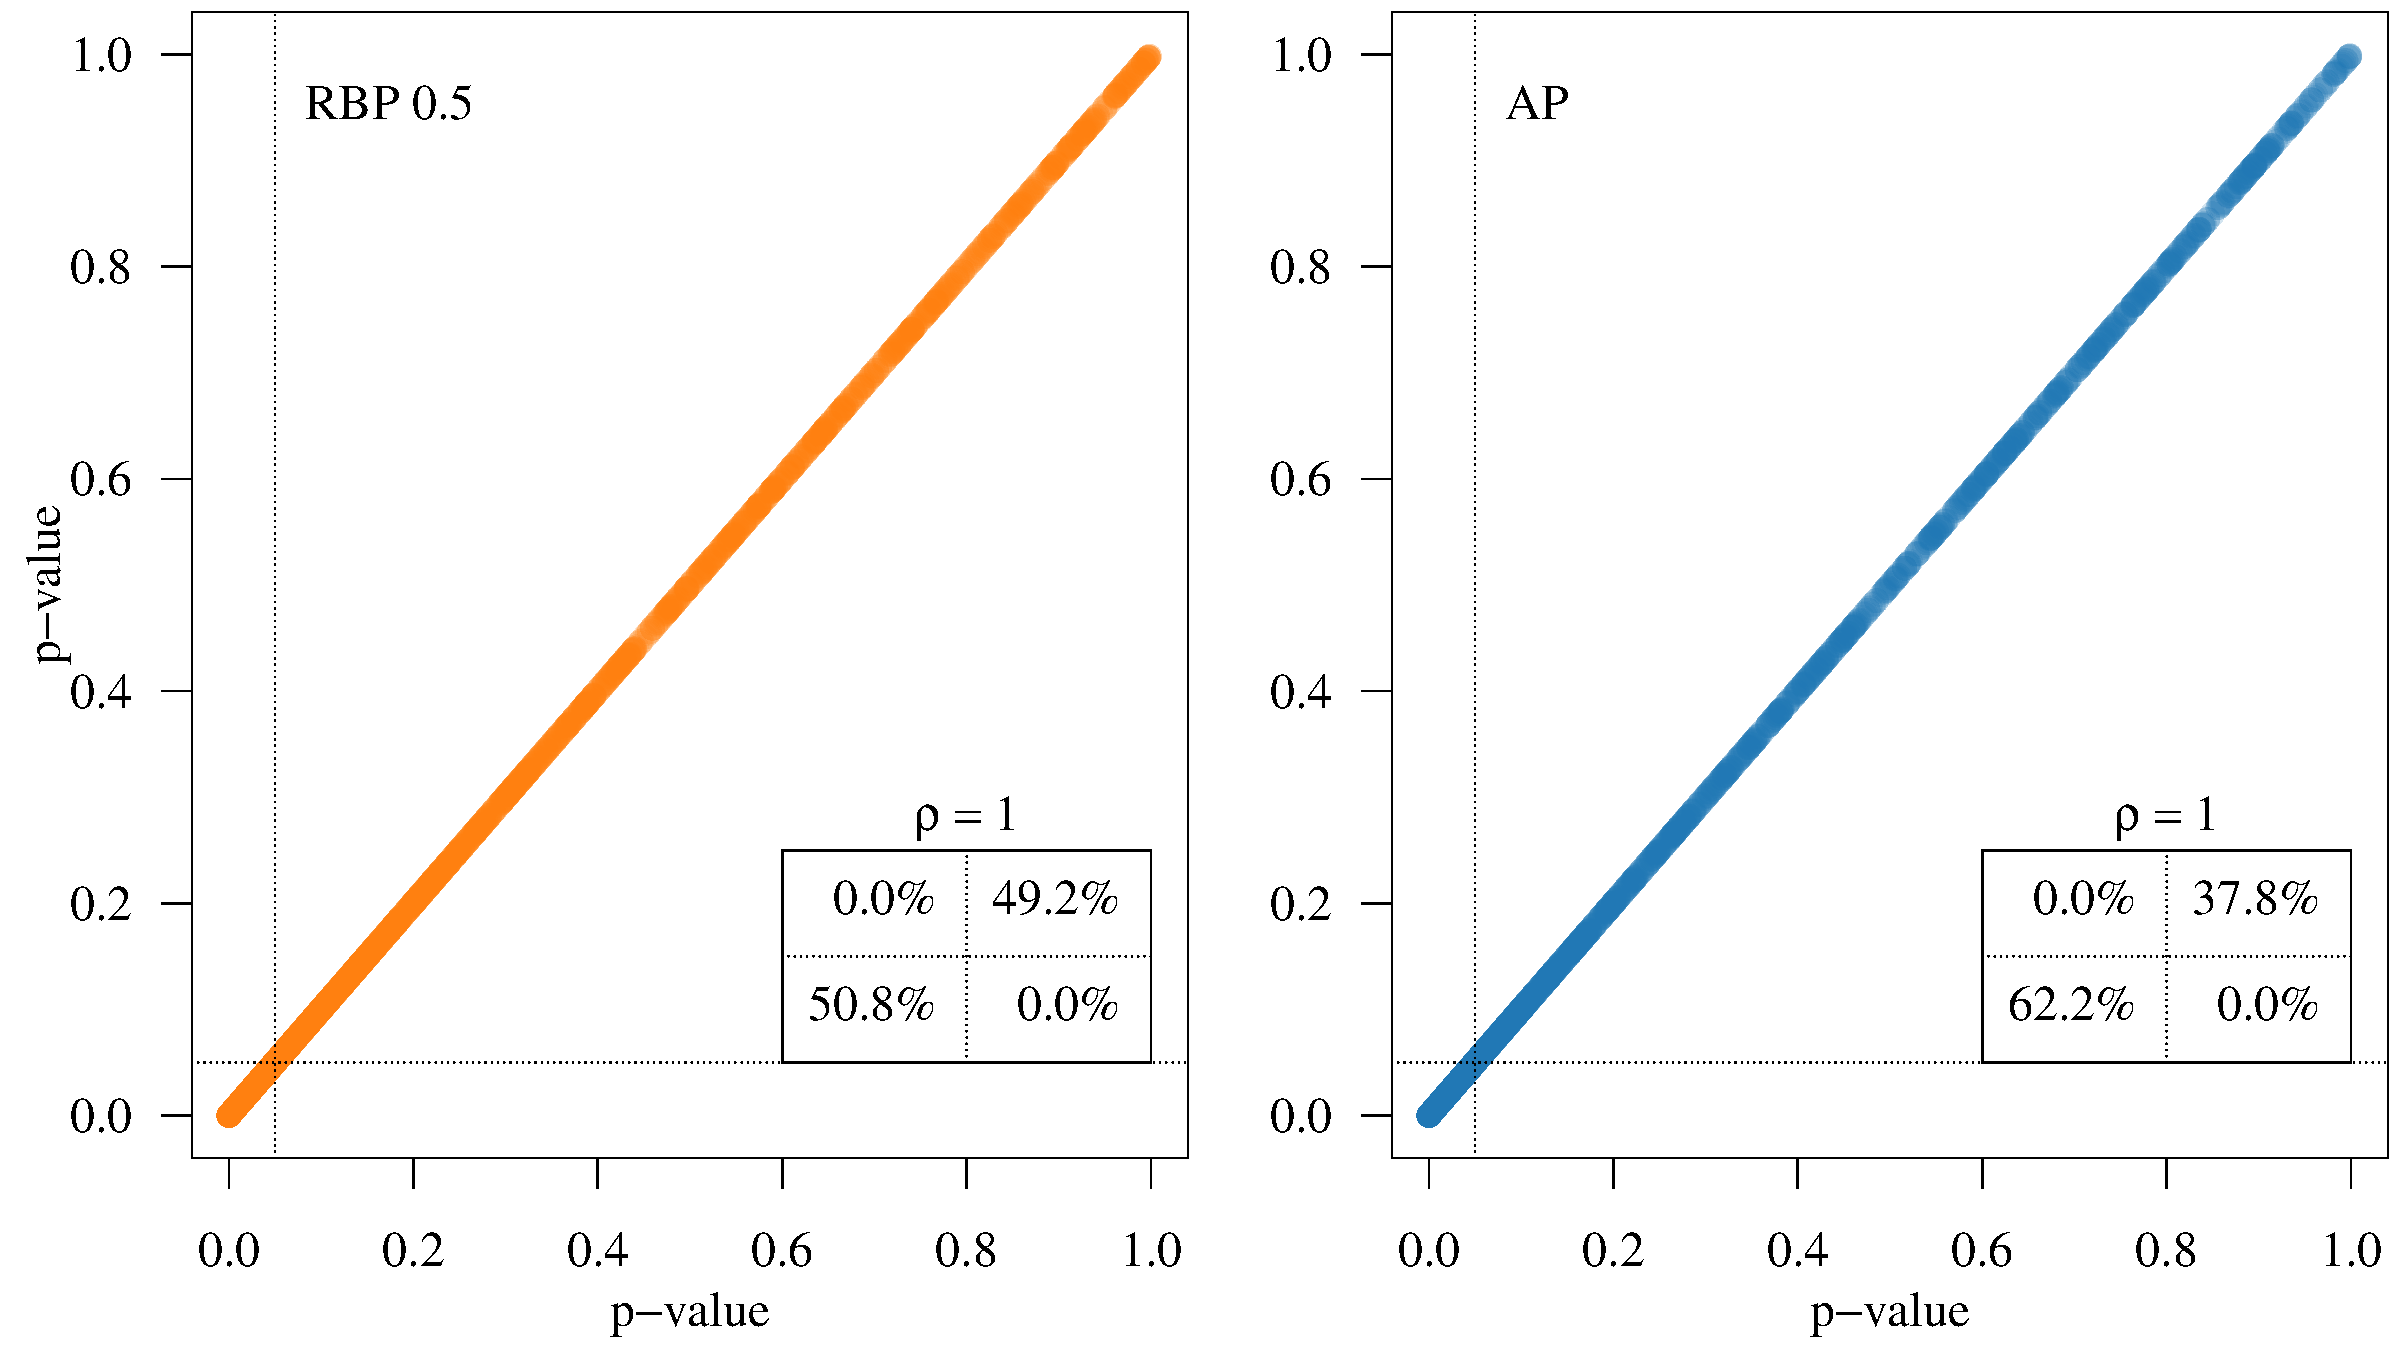
\includegraphics[width=0.98\textwidth, page=1]{figs/p_scatter_for_talk.pdf}
\end{frame}

\begin{frame}{Correlation of $p$ Values for All System Pairs}
\includegraphics[width=0.98\textwidth, page=3]{figs/p_scatter_for_talk.pdf}
\end{frame}

\begin{frame}{Correlation of $p$ Values for All System Pairs}
\includegraphics[width=0.98\textwidth, page=5]{figs/p_scatter_for_talk.pdf}
\end{frame}

\begin{frame}{Correlation of $p$ Values for All System Pairs}
\includegraphics[width=0.98\textwidth, page=6]{figs/p_scatter_for_talk.pdf}
\end{frame}

\begin{frame}{Correlation of $p$ Values for All System Pairs}
\includegraphics[width=0.98\textwidth, page=7]{figs/p_scatter_for_talk.pdf}
\end{frame}

\begin{frame}{Correlation of $p$ Values for All System Pairs}
\includegraphics[width=0.98\textwidth, page=11]{figs/p_scatter_for_talk.pdf}
\end{frame}

\begin{frame}{Summary}
Similarity score {\color{blue}ties} do have {\color{blue}potential} to affect system comparisons. But fortunately, {\color{blue}in practice}, they {\color{blue}did not}.\\[1.5em]

Allowing {\color{blue}deliberate introduction} of {\color{blue}ties} in runs by grouping rules resulted only {\color{blue}small changes} in the ability to {\color{blue}compare systems}. Reducing the accuracy of similarity scores to improve search speed and reduce space used is feasible.


\end{frame}
%-------------------

% \begin{frame}{How Similar Are They?}
%   \begin{table}
%   \parbox{.45\linewidth}{
%     \begin{tabular}{ccc}
%     student & Prof. S & Prof. T \\
%     \hline
%     A & 9.0 & 9.5 \\
%     B & 8.0 & 9.0 \\
%     C & 7.0 & 8.0 \\
%     D & 6.0 & 7.5 \\
%     E & 5.0 & 6.5 \\
%     \end{tabular}
%     \caption{Scores}
%     }
%    \parbox{.45\linewidth}{
%     \begin{tabular}{ccc}
%     student & Prof. S & Prof. T \\
%     \hline
%     A & 1 & 1 \\
%     B & 2 & 2 \\
%     C & 3 & 3 \\
%     D & 4 & 4 \\
%     E & 5 & 5 \\
%     \end{tabular}
%     \caption{Rankings}
%   }

%   \end{table}
%   \begin{itemize}
%   \item {
%     Two professors assess the presentations of five students. Do you think Prof. S and Prof. T agree with each other?
%   }
%   \end{itemize}
% \end{frame}

% \begin{frame}{How Similar Are Their Rankings?}
%   \begin{itemize}
%   \item {
%     How about Prof. U and Prof. V?
%   }
%   \end{itemize}
%   \begin{table}
%     \begin{tabular}{ccccc}
%     student & S & T & U & V\\
%     \hline
%     A & 1 & 1 & \alert{2} & 1\\
%     B & 2 & 2 & \alert{1} & 2\\
%     C & 3 & 3 & 3 & 3\\
%     D & 4 & 4 & 4 & \alert{5}\\
%     E & 5 & 5 & 5 & \alert{4}\\
%     \end{tabular}
%   \end{table}
%   \begin{itemize}
%   \item {
%     Is there any statistic which can measure the association between two orderings?
%   }
%   \end{itemize}
% \end{frame}
% \subsection{Correlation Measures}

% \begin{frame}{Kendall's $\tau$ (1955)}
%   \begin{itemize}
%   \item{
%     $X$ and $Y$ are two quantities (for example, Professors X and Y) which score \alert{a same set} of items (such as students).
%   }
%  \item{ Counts relative number of order concords versus discords }
%  \item All ranks treated equally
%  \item {$+1$ $\Rightarrow$ perfect correlate\\ \text{ } \text{0} $ \Rightarrow$ not correlate\\ $-1$ $\Rightarrow$ perfect inverse correlate}
%  \item But does this solve all the problems?
%   \end{itemize}
% \end{frame}

% \subsection{Why we need this?}
% \begin{frame}{Why this?}
%   \includegraphics[width=0.98\textwidth]{system_run_diagram.pdf}
%   \begin{itemize}
%   \item The effectiveness of Information Retrieval system can be measured by a variety of proposed evaluation metrics such as AP, Prec@$k$, NDCG@$k$, RBP@$p$, INSQ, ERR etc.
%   \end{itemize}
% \end{frame}

% \begin{frame}{Why this?}
% \begin{itemize}
% \item  Metrics Selecting Problems:
%   \begin{itemize}
%   \item Which metrics should be selected for IR evaluation?
%   \item Which of selected metrics can be trust if they produce opposite conclusion?
%   \end{itemize} 
% \item Discover user models behind metrics, correlation of metrics,...\\[1em]

% \item Problematic properties:
%   \begin{itemize}
%   \item Top-weighted, interested a fidelity at early ranks
%   \item Handling ties.
%   \item May even be over non-conjoint sets
%   \end{itemize}
% \item  Kendall's $\tau$ or Spearman's $\rho$ is no longer qualified.
% \end{itemize}  
% \end{frame}


% \begin{frame}{Are they highly correlated?}
% \includegraphics[height=0.5\textheight]{NDCG-AP-rank-R03.pdf}
% \pause
% \includegraphics[height=0.5\textheight]{NDCG-RBP-rank-R03.pdf}\\
% \pause
% \parbox{.5\linewidth}{
% \begin{itemize}
% \item NDCG-AP: 
% \begin{align*}
% \tau=0.895\\
% \rho=0.984
% \end{align*}
% \end{itemize}
% }\parbox{.5\linewidth}{
% \begin{itemize}
% \item NDCG-RBP: 
% \begin{align*}
% \tau=0.566\\
% \rho=0.766
% \end{align*}
% \end{itemize}
% }
% \end{frame}

% \begin{frame}{Top-weighted Rank Correlation Measures}
% \alert{Rank Biased Overlap (RBO)} proposed by Webber et al.
% \begin{itemize}
% \item models a stochastic user examining two ranked lists $L_1$ and $L_2$ from the top to the bottom ranks.
% \begin{itemize}
% \item Denote $S(L,d)$ as the set that contains all the items ranked from depth 1 to $d$ in $L$.
% \item The \alert{overlap} of $L_1$ and $L_2$, at depth $d$: $O(L_1, L_2, d)=S(L_1,d)\cap S(L_2,d). $
% \item When there are \alert{no ties}, the \alert{agreement} is computed as $A(L_1, L_2, d)=|O(L_1,L_2,d)|/d. $
% \end{itemize}
% \item geometric sequence of weights, $(1-p)p^{k-1}$, are applied to agreement of depth $k$, for all $k$.
% \item RBO is the expected average agreement of two ranked lists.
% \item RBO of 1 is perfect agreement; RBO of 0 is no agreement.
% \end{itemize}
% \end{frame}

% \begin{frame}{Are they highly correlated?}
% \includegraphics[height=0.5\textheight]{NDCG-AP-rank-R03.pdf}
% \includegraphics[height=0.5\textheight]{NDCG-RBP-rank-R03.pdf}\\
% \parbox{.5\linewidth}{
% \begin{itemize}
% \item NDCG-AP: 
% \begin{align*}
% &\tau=0.895 \text{ }\rho=0.984\\
% &\\
% &\\
% &\\
% \end{align*}
% \end{itemize}
% }\parbox{.5\linewidth}{
% \begin{itemize}
% \item NDCG-RBP: 
% \begin{align*}
% &\tau=0.566 \text{ }\rho=0.766\\
% &\\
% &\\
% &\\
% \end{align*}
% \end{itemize}
% }
% \end{frame}

% \begin{frame}{Are they highly correlated?}
% \includegraphics[height=0.5\textheight]{NDCG-AP-rank-R03.pdf}
% \includegraphics[height=0.5\textheight]{NDCG-RBP-rank-R03.pdf}\\
% \parbox{.5\linewidth}{
% \begin{itemize}
% \item NDCG-AP: 
% \begin{align*}
% &\tau=0.895 \text{ } \rho=0.984\\
% &\alert{\text{RBO}(p=0.75)=0.946}\\
% &\\
% &\\
% \end{align*}
% \end{itemize}
% }\parbox{.5\linewidth}{
% \begin{itemize}
% \item NDCG-RBP: 
% \begin{align*}
% &\tau=0.566 \text{ } \rho=0.766\\
% &\alert{\text{RBO}(p=0.75)=2.092e-13}\\
% &\\
% &\\
% \end{align*}
% \end{itemize}
% }
% \end{frame}

% \begin{frame}{Are they highly correlated?}
% \includegraphics[height=0.5\textheight]{NDCG-AP-rank-R03-1024.png}
% \includegraphics[height=0.5\textheight]{NDCG-RBP-rank-R03-1024.png}\\
% \parbox{.5\linewidth}{
% \begin{itemize}
% \item NDCG-AP: 
% \begin{align*}
% &\tau=0.895 \text{ }\rho=0.984\\
% &\text{RBO}(p=0.75)=0.946\\
% &\alert{\text{RBO}(p=0.999)=0.890}\\
% &\\
% \end{align*}
% \end{itemize}
% }\parbox{.5\linewidth}{
% \begin{itemize}
% \item NDCG-RBP: 
% \begin{align*}
% &\tau=0.566 \text{ } \rho=0.766\\
% &\text{RBO}(p=0.75)=2.092e-13\\
% &\alert{\text{RBO}(p=0.999)=0.402}\\
% &\\
% \end{align*}
% \end{itemize}
% }
% \end{frame}

% \begin{frame}{Are they highly correlated?}
% \includegraphics[height=0.5\textheight]{NDCG-AP-rank-R03-2048.png}
% \includegraphics[height=0.5\textheight]{NDCG-RBP-rank-R03-2048.png}\\
% \parbox{.5\linewidth}{
% \begin{itemize}
% \item NDCG-AP: 
% \begin{align*}
% &\tau=0.895 \text{ }\rho=0.984\\
% &\text{RBO}(p=0.75)=0.946\\
% &\text{RBO}(p=0.999)=0.890\\
% &\alert{\text{RBO}(p=0.9995)=0.917}
% \end{align*}
% \end{itemize}
% }\parbox{.5\linewidth}{
% \begin{itemize}
% \item NDCG-RBP: 
% \begin{align*}
% &\tau=0.566 \rho=0.766\\
% &\text{RBO}(p=0.75)=2.092e-13\\
% &\text{RBO}(p=0.999)=0.402\\
% &\alert{\text{RBO}(p=0.9995)=0.582}
% \end{align*}
% \end{itemize}
% }
% \end{frame}

% \begin{frame}{How does RBO handle ties?}
%  \begin{table}
%   \parbox{.25\linewidth}{
%     \begin{tabular}{ccc}
%     item & $M_1$ & $M_2$ \\
%     \hline
%     A & 9.5 & 9.0\\
%     B & \alert{8.0} & 8.0\\
%     C & \alert{8.0} & \alert{7.5}\\
%     D & 7.5 & \alert{7.5}\\
%     E & 6.5 & \alert{7.5}\\
%     \end{tabular}
%   }
%   \parbox{.72\linewidth}{
%     \begin{tabular}{cccll}
%     depth & $M_1$ & $M_2$ & $S(M_1,d)$ & $S(M_2,d)$\\
%     \hline
%     1 & A & A &\{A\}& \{A\}\\
%     2 & \multirow{2}{*}{\bigg\{\alert{B,C}} & B& \{A,\alert{B,C}\} & \{A,B\}\\
%     3 &  & \multirow{3}{*}{\Bigg\{\alert{C,D,E}}& \{A,\alert{B,C}\} & \{A,B,\alert{C,D,E}\}\\
%     4 & D & &\{A,B,C,D\} & \{A,B,\alert{C,D,E}\}\\
%     5 & E & &\{A,B,C,D,E\} & \{A,B,\alert{C,D,E}\}
%     \end{tabular}
%   }
% \end{table}
% \begin{itemize}
% \item When there are ties, the agreement of depth $d$ is refined as:
% \end{itemize}
% \begin{align*}
% A(L_1,L_2,d) =\frac{2 \cdot |O(L_1,L_2,d)|}{|S(L_1,d)| + |S(L_2,d)|}.
% \end{align*}
% For example, $A(M_1,M_2,3) =2 \cdot 3/(3 + 5)=6/8.$
% \end{frame}

% \begin{frame}{Ranking of Ties}
%  \begin{itemize}
%  \item Note that ties handling strategy proposed by Webber et al. assumes that items with \alert{same score values} should be place at the the \alert{same rank}.
%  \item But a philosophical question arise -- if items \alert{must be linearized for sequential presentation}, there will be \alert{$n!$} different possible orders for ranking \alert{$n$} items that have same score values.
% \item In the example above, C, D and E can be ranked in one of 6 orders.
%  \end{itemize}
%   \begin{table}
%   \parbox{.35\linewidth}{
%     \begin{tabular}{ccc}
%     \toprule
%     depth & $M_1$ & $M_2$\\
%     \midrule
%     1 & A & A \\
%     2 & \multirow{2}{*}{\bigg\{\alert{B,C}} & B \\
%     3 &  & \multirow{3}{*}{\Bigg\{\alert{C,D,E}}\\
%     4 & D & \\
%     5 & E &\\
%     \bottomrule
%     \end{tabular}
%     }\pause \parbox{.03\linewidth}{$\Rightarrow$} \parbox{.3\linewidth}{
%     \begin{tabular}{ccc}
%      \toprule
%     depth & $M_1$ & $M_2$ \\
%     \midrule
%     1 & A & A\\
%     2 & B & B\\
%     3 & C & \alert{C}\\
%     4 & D & \alert{D}\\
%     5 & E & \alert{E}\\
%     \bottomrule
%     \end{tabular}
%   }\pause \parbox{.3\linewidth}{
%     \begin{tabular}{ccc}
%      \toprule
%     depth & $M_1$ & $M_2$ \\
%     \midrule
%     1 & A & A\\
%     2 & B & B\\
%     3 & C & \alert{E}\\
%     4 & D & \alert{C}\\
%     5 & E & \alert{D}\\
%     \bottomrule
%     \end{tabular}
%   }
% \end{table}
% \end{frame}




% \begin{frame}{}
% \begin{table}
% \parbox{1.1\linewidth}{
%  \begin{tabular}{clll}
%  \toprule
%  $d$ & $S(M_1,d)$ & $S(M_2,d)$ & $O(M_1,M_2,d)$  \\
%   \midrule
%   1 & 1A & 1A & 1A \\[0.5em]
%   2 & 1A, $\frac{1}{2}$B, $\frac{1}{2}$C & 1A, 1B &  1A, $\frac{1}{2}$B \\[0.5em]
%   3 & 1A, 1B, 1C & 1A, 1B, $\frac{1}{3}$C,$\frac{1}{3}$D,$\frac{1}{3}$E & 1A, 1B, $\frac{1}{3}$C \\[0.5em]
%   4 & 1A, 1B, 1C, 1D & 1A, 1B, $\frac{2}{3}$C, $\frac{2}{3}$D, $\frac{2}{3}$E & 1A, 1B, $\frac{2}{3}$C, $\frac{2}{3}$D \\[0.5em]
%   5 & 1A, 1B, 1C, 1D, 1E & 1A, 1B, 1C, 1D, 1E & 1A, 1B, 1C, 1D, 1E \\
%   \bottomrule
%   \end{tabular}
%   }\\[1.1em]
% \end{table}

% \begin{tabular}{cccll}
%     \toprule
%     depth & $M_1$ & $M_2$ \\
%     \midrule
%     1 & A & A \\
%     2 & \multirow{2}{*}{\bigg\{\alert{B,C}} &B \\
%     3 &  & \multirow{3}{*}{\Bigg\{\alert{C,D,E}}\\
%     4 & D & \\
%     5 & E & \\
%     \bottomrule
% \end{tabular}
% \\[1.2em]

% \end{frame}


% \begin{frame}
% \begin{table}
%  \begin{tabular}{clll}
%  \toprule
%  $d$ & $S(M_1,d)$ & $S(M_2,d)$ & $O(M_1,M_2,d)$  \\
%   \midrule
%   1 & 1A & 1A & 1A \\[0.5em]
%   2 & 1A, $\frac{1}{2}$B, $\frac{1}{2}$C & 1A, 1B &  1A, $\frac{1}{2}$B \\[0.5em]
%   3 & 1A, 1B, 1C & 1A, 1B, $\frac{1}{3}$C,$\frac{1}{3}$D,$\frac{1}{3}$E & 1A, 1B, $\frac{1}{3}$C \\[0.5em]
%   4 & 1A, 1B, 1C, 1D & 1A, 1B, $\frac{2}{3}$C, $\frac{2}{3}$D, $\frac{2}{3}$E & 1A, 1B, $\frac{2}{3}$C, $\frac{2}{3}$D \\[0.5em]
%   5 & 1A, 1B, 1C, 1D, 1E & 1A, 1B, 1C, 1D, 1E & 1A, 1B, 1C, 1D, 1E \\
%   \bottomrule
%   \end{tabular}
% \end{table}
% \begin{align*}
% A(M_1,M_2,1)&=1/1=1\\
% A(M_1,M_2,2)&=(1+\frac{1}{2})/2=3/4\\
% A(M_1,M_2,3)&=(1+1+\frac{1}{3})/3=7/9\\
% A(M_1,M_2,4)&=(1+1+\frac{2}{3}+\frac{2}{3})/4=10/12\\
% A(M_1,M_2,5)&=(1+1+1+1+1)/5=1\\
% \end{align*}

% \end{frame}

% \begin{frame}{Want to Know More?}
% \centering
% Please read my Report.\\[2em]

% There isn't time here!
% \end{frame}


% \begin{frame}{Summary}
% \begin{itemize}
% \item Traditional ranked correlation coefficients are NOT top-weighted
% \item Rank Biased Overlap is a top-weighted measure, but does it handle ties in a manner that reflects sequential processing.
% \item We have developed an alternative probabilistic calculation
% \item The next step is to apply it to systems and metrics as part of a full-scale IR investigation.
% \item Maybe can help end some arguments in IR community.
% \end{itemize}
% \end{frame}

% All of the following is optional and typically not needed. 

\end{document}


